\section*{Lezione 4}
\addcontentsline{toc}{section}{Lezione 4}

Seguendo l'esempio dei codici rettangolari, proviamo a disporre ora i bit di messaggio in altre forme logiche, in modo da coprire il più gran numero di bit di messaggio con ogni bit di controllo.

\subsection*{Codici triangolari - 1 Errore}
\addcontentsline{toc}{subsection}{Codici triangolari}
Proviamo a creare una forma logica di un codice triangolare:

\begin{equation*}
\begin{matrix}
\textit{o} & \textit{o} & \textit{o} & \textit{o} & x\\
\textit{o} & \textit{o} & \textit{o} & x\\
\textit{o} & \textit{o} & x\\
\textit{o} & x\\
x
\end{matrix}
\end{equation*}

Ovviamente il numero di bit di messaggio deve consentire una costruzione di questo genere (dagli antichi greci: numeri triangolari).

Come prima, ogni bit di controllo copre la relativa colonna e riga.

Quanto vale la ridondanza di questo tipo di codici?

Il numero di bit totali è 
\begin{equation}
\sum_{i=1}^{n}i = \frac{n(n+1)}{2}
\end{equation}
mentre il numero di bit di messaggio è
\begin{equation}
\sum_{i=1}^{n-1}i = \frac{(n-1)(n-1+1)}{2} = \frac{(n-1)n}{2}
\end{equation}

Per cui passiamo a calcolare la ridondanza:

\begin{equation}
R_{triangolare} = \frac{\frac{n(n+1)}{2}}{\frac{(n-1)n}{2}}
\end{equation}
\begin{equation*}
= \frac{\cancel{n}(n+1)}{\cancel{2}} \cdot \frac{\cancel{2}}{(n-1)\cancel{n}}
\end{equation*}
\begin{equation*}
= \frac{(n+1)}{(n-1)}
\end{equation*}
\begin{equation*}
= \frac{(n-1) + 2}{(n-1)}
\end{equation*}
\begin{equation*}
= 1 + \frac{2}{(n-1)}
\end{equation*}

\newpage

Da qui, l'eccesso di ridondanza vale

\begin{equation}
\frac{2}{(n-1)}
\end{equation}

Confrontiamolo con l'eccesso di ridondanza dei codici quadrati:

\begin{equation*}
ecc_{quadrato} = \frac{2}{n-1}+\frac{1}{(n-1)^2}
\end{equation*}
\begin{equation*}
ecc_{triangolo} = \frac{2}{n-1}
\end{equation*}

Si nota ovviamente come i codici triangolari siano sicuramente più efficienti.

\subsection*{Codici cubici - 1 Errore}
\addcontentsline{toc}{subsection}{Codici cubici}

Un'altra disposizione che si può seguire per ordinare i bit di messaggio è a forma cubica.

\begin{figure}[h]
	\centering
	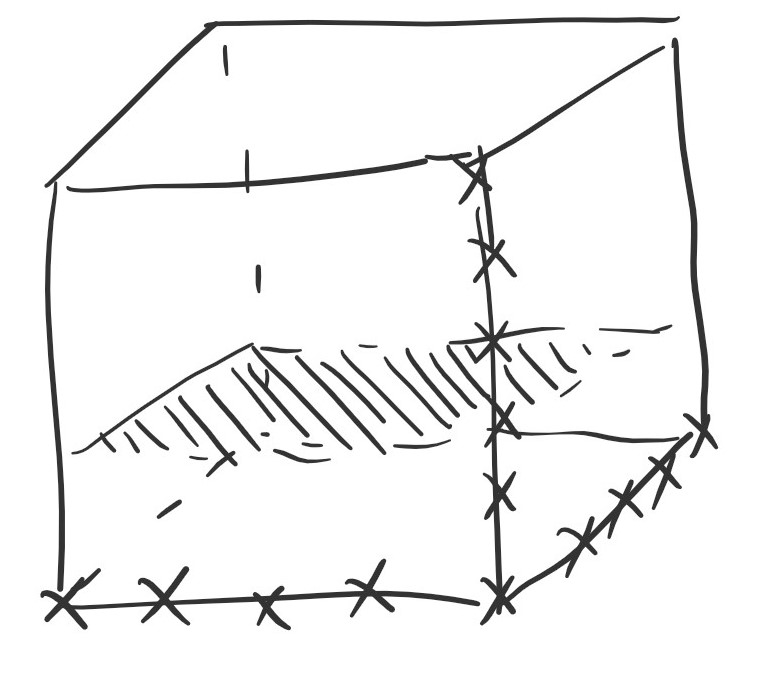
\includegraphics[width=0.6\linewidth]{immagini/img5}
\end{figure}

Facendo dei conti \textit{a spanne}, ci sono $n^3$ posizioni, le cifre di controllo sono $3(n-1) + 1 = 3n-2$.

La ridondanza più o meno quindi vale

\begin{equation}
R = \frac{(n-1)^3+3n-2}{(n-1)^3} \approx 1 + \frac{3}{n^2}
\end{equation}

Seguendo questo ragionamento, potrei pensare di aumentare le dimensioni

\subsection*{Codici ipercubici}
\addcontentsline{toc}{subsection}{Codici ipercubici}

Seguendo il modello dei \textit{conti a spanne}, diciamo più o meno che le cifre di messaggi è $(n-1)^4$, mentre le check digit saranno $4(n-1)+1=4n-3$.

La ridondanza quindi varrà:

\begin{equation}
R = 1 + \frac{4n-3}{(n-1)^4} \approx 1 + \frac{4}{n^3}
\end{equation}

Da qui si nota come si può passare a ragionare in \textit{k} dimensioni, e si possono tirare delle conclusioni:

\begin{equation}
(n-1)^k \; \; \; \text{bit di messaggio}
\end{equation}
\begin{equation*}
k(n-1)+1 = kn-k+1 \; \; \; \text{bit di controllo}
\end{equation*}
\begin{equation*}
R = 1 + \frac{kn-k+1}{(n-1)^k} \approx 1 + \frac{k}{n^{k-1}} \; \; \; \text{ridondanza}
\end{equation*}

\smallskip

Da qui si nota come la ridondanza decresce in maniera polinomiale, possiamo fare di meglio?

\subsection*{Codici di Hamming}
\addcontentsline{toc}{subsection}{Codici di Hamming}

Codici ottimali per individuare e correggere 1 errore (al massimo) in un canale caratterizzato da rumore bianco.
Cosa significa codici ottimali? Il rapporto fra cifre di controllo e cifre di messaggio è esponenziale, meglio di così non si può fare.

Da ora in poi ci riferiremo con \textit{k} alle cifre di messaggio, \textit{m} alle cifre di controllo. \textit{n} sarà la loro somma.

Le combinazioni (configurazioni) di cifre di controllo sono $2^m$.
Da notare come deve sempre valere $2^m \geq n+1$, questo è necessario in quanto ci dev'essere una configurazione per ogni posizione di errore, più uno (configurazione per rappresentare zero errori).
Altrimenti non abbiamo abbastanza configurazioni per rappresentare tutte le situazioni (errore in posizione 3, errore in posizione 8, ecc).\\

Supponiamo di voler mandare un messaggio di 7 bit, ci chiediamo quanti di questi bit possono essere di messaggio e quanti di controllo?

\begin{equation*}
2^m \geq 8 \rightarrow m \geq 3 \rightarrow m=3
\end{equation*}
\begin{equation*}
k = 7 - 3 = 4
\end{equation*}

\newpage

Oppure posso chiedermi: devo inviare 4 cifre di messaggio sul canale, di quante cifre di controllo ho bisogno?

\begin{equation*}
2^m \geq n+1 \rightarrow 2^m \geq m+k+1 \rightarrow 2^m \geq m+5
\end{equation*}

Quando è vero $2^m \geq m+5$? Proviamo ad assegnare dei valori a \textit{m}:

\begin{table}[h]
	\centering
	\begin{tabular}{l|l|l}
		$m$ & $2^m$ & $m+5$ \\
		\hline
		1   & 2     & 6     \\
		2   & 4     & 7     \\
		3   & 8     & 8     \\
		4   & 16    & 9    
	\end{tabular}
\end{table}

Il valore più piccolo che ci va bene è proprio 3, quindi l'ideale è utilizzare 3 cifre di controllo.

Ciascuna cifra di controllo fa il controllo di parità su diverse cifre di messaggio. Facciamo un esempio:\\
Ho 9 cifre di messaggio, avrò quindi 3 cifre di controllo, come si suddividono le cifre per il calcolo delle parità?


\begin{equation}
c_1 = x_1 \oplus x_2 \oplus x_5 \oplus x_7
\end{equation}
\begin{equation*}
c_2 = x_5 \oplus x_7 \oplus x_8 \oplus x_9
\end{equation*}
\begin{equation*}
c_3 = x_1 \oplus x_2 \oplus x_8 \oplus x_9
\end{equation*}

Ma quanto vale la somma di $c_1$ e $c_2$ (ricordando che $x \oplus 0 = x$)?

\begin{equation*}
c_1 \oplus c_2 = x_1 \oplus x_2 \oplus x_8 \oplus x_9
\end{equation*}

che è esattamente uguale a $c_3$!

Allo stesso modo considerando vettori binari di \textit{n} elementi, una somma in modulo due e un prodotto modulo due, posso effettuare il calcolo in questo modo:

\begin{equation}
v_1 = (1,1,0,0,1,0,1,0,0)
\end{equation}
\begin{equation*}
v_2 = (0,0,0,0,1,0,1,1,1)
\end{equation*}
\begin{equation*}
\downarrow
\end{equation*}
\begin{equation*}
v_1 + v_2 = (1,1,0,0,0,0,0,1,1) \; \; \; \; \; \; \; \, \,
\end{equation*}


Questo insieme, composto da ($\{0,1\}^n, +_2, \cdot$) è uno spazio vettoriale, quindi le tre equazioni di parità considerate sono linearmente dipendenti, e questo ovviamente è da evitare visto che la terza equazione non da informazione in quanto è ricavabile dalle altre due.

\newpage 

Ripendendo l'esempio del pacchetto di 7 bit, scriviamo questa tabella che rappresenta le posizioni:

\begin{table}[h]
	\centering
	\begin{tabular}{l|l}
		pos & pos in binario \\
		\hline
		1   & 001            \\
		2   & 010            \\
		3   & 011            \\
		4   & 100            \\
		5   & 101            \\
		6   & 110            \\
		7   & 111        \\
		0 (nessun errore) & 000    
	\end{tabular}
\end{table}

Da notare come i bit necessari per coprire tutte le posizioni sono 3, esattamente come il numero di bit di controllo.
L'insieme delle posizioni in valore binario assume il nome di \textit{sindrome}.
Se la sindrome vale 101 allora è avvenuto un errore in posizione 5.
Non ci resta che capire come assegnare le posizioni per ogni bit.

Definiamo le cifre di controllo come le colonne della tabella precedente, quindi:

\begin{table}[h]
	\centering
	\begin{tabular}{l|lll}
		\hline
		1   & 0 & 0 & 1            \\
		2   & 0 & 1 & 0            \\
		3   & 0 & 1 & 1            \\
		4   & 1 & 0 & 0            \\
		5   & 1 & 0 & 1            \\
		6   & 1 & 1 & 0            \\
		7   & 1 & 1 & 1        \\
		\hline
		& $c_3$ & $c_2$ & $c_1$    
	\end{tabular}
\end{table}

Supponiamo che sia avvenuto un errore in posizione 5, quindi la terza e la prima cifra di controllo devono 'attivarsi', quindi valere 1, mentre la seconda deve rimanere a 0 (in questo modo il valore è 101 che rappresenta la posizione 5).\\
Quindi il bit numero 5 deve far parte delle equazioni che calcolano $c_3$ e $c_1$, e non deve far parte dell'equazione che calcola $c_2$.
Per calcolare $c_1$ quindi, mi basta vedere su che posizioni ci sono degli 1, nel nostro esempio calcoleremo:
\begin{itemize}
	\item $c_1$ sfruttando le posizioni 1, 3, 5 e 7
	\item $c_2$ sfruttando le posizioni 2, 3, 6 e 7
	\item $c_3$ sfruttando le posizioni 4, 5, 6 e 7
\end{itemize}

Quindi sfruttando queste \textit{c}, se avviene un errore in posizione 5, la tripla varrà 101, visto che la posizione 5 è inclusa in $c_1$ e in $c_3$.

Le equazioni così formate saranno linearmente indipendenti (dimostrazione balza).

In generale le cifre di controllo vengono posizionate seguendo il primo numero che codificano, quindi:

\begin{itemize}
	\item $c_1$ in posizione 1
	\item $c_2$ in posizione 2
	\item $c_3$ in posizione 4
\end{itemize}

Quest'ordine, al crescere delle cifre di messaggio, crescerà seguendo l'ordine di $2^n$ (quindi posizione 1, 2, 4, 8, 16...).\\
Da notare come la distanza fra una cifra di controllo e l'altra cresce in maniera esponenziale, questo a confermare il fatto che i codici di hamming sono ottimali.

Vediamo un esempio:
\begin{itemize}
	\item Messaggio di 4 bit: \texttt{0110}
	\item $k=4$
\end{itemize}
Sfruttando la disequazione $2^m \geq \underset{n}{m+k}+1$, otteniamo che $m=3$, quindi il numero totale di bit sarà 4+3.\\
Ora disponiamo le cifre di controllo, ricordando che la loro posizione vale $2^i$ con $i$ che parte a 0 a $m$.

\begin{equation*}
1 \; \; \; \; 2 \; \; \; \; 3  \; \; \; \; 4  \; \; \; \; 5  \; \; \; \; 6  \; \; \; \; 7
\end{equation*}
\begin{equation*}
c_1 \; \;  \; c_2 \; \; \; \; \;  \; \; \; c_3  \; \; \; \; \; \; \; \; \; \; \; \; \; \; \; \; \; 
\end{equation*}

Quindi le 4 cifre di messaggio verranno distribuite lungo le posizioni rimanenti:

\begin{equation*}
1 \; \; \; \; \; 2 \; \; \; \; \; 3  \; \; \; \; \; 4  \; \; \; \; \; 5  \; \; \; \; \; 6  \; \; \; \; \; 7
\end{equation*}
\begin{equation*}
c_1 \; \; \; c_2 \; \; \; m_1 \; \; \;  c_3  \; \; \; m_2 \; \; \; m_3 \; \; \; m_4
\end{equation*}

A questo punto si passa a calcolare il valore delle varie $c_i$ in questo modo:

\begin{equation*}
c_1 \oplus m_1 \oplus m_2 \oplus m_4 = 0
\end{equation*}
\begin{equation*}
c_2 \oplus m_1 \oplus m_3 \oplus m_4 = 0
\end{equation*}
\begin{equation*}
c_3 \oplus m_2 \oplus m_3 \oplus m_4 = 0
\end{equation*}

In ogni riga il $c_i$ viene calcolato in modo da avere un numero pari di 1.

Il messaggio per ora è uguale a:

\begin{equation*}
c_1 \; c_2 \; 0 \; c_3 \; 1 \; 1 \; 0
\end{equation*}

Quindi passo al calcolo di $c_1$:

\begin{equation*}
\text{parity}(c_1 \; 0 \; 1 \; 0) = 0
\end{equation*}

Per avere parità pari $c_1$ deve valere 1, quindi il messaggio diventa:

\begin{equation*}
1 \; c_2 \; 0 \; c_3 \; 1 \; 1 \; 0
\end{equation*}

E così via per le altre due cifre di controllo:

\begin{equation*}
\text{parity}(c_2 \; 0 \; 1 \; 0) = 0
\end{equation*}
\begin{equation*}
\downarrow
\end{equation*}
\begin{equation*}
c_2 = 1
\end{equation*}
\vspace{5mm}
\begin{equation*}
\text{parity}(c_3 \; 1 \; 1 \; 0) = 0
\end{equation*}
\begin{equation*}
\downarrow
\end{equation*}
\begin{equation*}
c_3 = 0
\end{equation*}
Il messaggio che verrà inviato nel canale sarà quindi:
\begin{equation*}
1100110
\end{equation*}

Quando il mittente riceve il messaggio, dovrà controllare se sono avvenuti degli errori.
Il messaggio, abbiamo detto, è così composto:
\begin{equation*}
c_1 \; c_2 \; 0 \; c_3 \; 1 \; 1 \; 0
\end{equation*}
Il mittente calcolerà il valore della sindrome controllando le parità delle varie posizioni, un trucco per vedere visivamente in che modo vengono effettuati i calcoli è il seguente:

\begin{figure}[h]
	\centering
	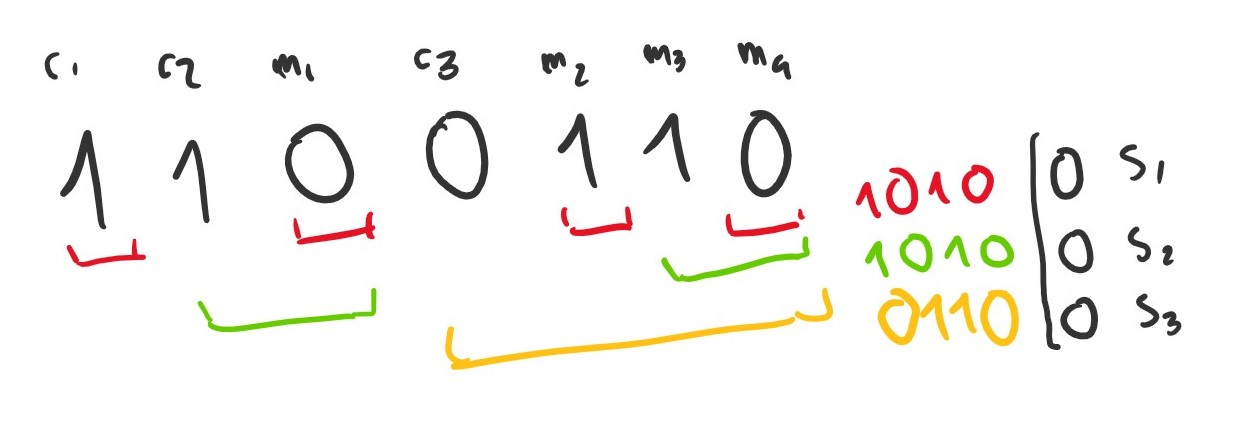
\includegraphics[width=0.7\linewidth]{immagini/img6}
\end{figure}

Quindi partendo dalla fine, il primo bit della sindrome viene calcolando facendo la parità sull'ultima cifra, terz'ultima e così via scalando sempre di 1, il secondo bit invece ne prende due alla volta e scala di due, il terzo ne prende quattro e scala di quattro. Seguendo sempre quindi lo schema di $2^n$.

\newpage

Se capitasse un errore?
Mettiamo che avvenga un errore in posizione 5, il messaggio passa da:

\begin{equation*}
1 \; 1 \; 0 \; 0 \; 1 \; 1 \; 0
\end{equation*}

a

\begin{equation*}
1 \; 1 \; 0 \; 0 \; \textbf{0} \; 1 \; 0
\end{equation*}

La cosa che farà il mittente sarà quindi quello di calcolare la sindrome.

\begin{equation*}
s_1 = \text{parity}(1000) = 1
\end{equation*}
\begin{equation*}
s_2 = \text{parity}(1010) = 0
\end{equation*}
\begin{equation*}
s_3 = \text{parity}(0010) = 1
\end{equation*}

Il valore finale sarà quindi $s_1 \; s_2 \; s_3$ uguale a 101, quindi il mittente riconosce che è avvenuto un errore in posizione 5.

E se la cifra modificata fosse di controllo? Proviamo con la seconda cifra:

\begin{equation*}
1 \; \textbf{0} \; 0 \; 0 \; 1 \; 1 \; 0
\end{equation*}

Calcolo della sindrome:

\begin{equation*}
s_1 = \text{parity}(1010) = 0
\end{equation*}
\begin{equation*}
s_2 = \text{parity}(0010) = 1
\end{equation*}
\begin{equation*}
s_3 = \text{parity}(0110) = 0
\end{equation*}

Quindi questo tipo di codici riconosce errori anche sulle cifre di controllo!
Ma nel caso di due errori nel messaggio? 
Proviamo a modificare due cifre del pacchetto:

\begin{equation*}
1 \; \textbf{0} \; 0 \; 0 \; \textbf{0} \; 1 \; 0
\end{equation*}

Calcolo della sindrome:

\begin{equation*}
s_1 = \text{parity}(1000) = 1
\end{equation*}
\begin{equation*}
s_2 = \text{parity}(0010) = 1
\end{equation*}
\begin{equation*}
s_3 = \text{parity}(0010) = 1
\end{equation*}

Essa dice che è avvenuto un errore in posizione 7, cosa falsa.
Si noti quindi come il codice di Hamming copre un singolo errore, nel caso di errori multipli essi non sono riconoscibili.

\newpage 

Come si gestisce il caso di 4 cifre di controllo?

\begin{equation*}
m=4
\end{equation*}
\begin{equation*}
2^m \geq n+1
\end{equation*}
\begin{equation*}
16 \geq n+1
\end{equation*}
\begin{equation*}
n \leq 15
\end{equation*}
\begin{equation*}
n = 15 \; (\text{ottimale})
\end{equation*}
\begin{equation*}
k=n-m=15-4=11
\end{equation*}

Vediamo come si distribuiscono le cifre di controllo nel messaggio:

\begin{table}[h]
	\centering
	\begin{tabular}{|l|l|l|l|l|l|l|l|l|l|l|l|l|l|l|}
		\hline
		$c_1$ & $c_2$ & $m_1$ & $c_3$ & $m_2$ & $m_3$ & $m_4$ & $c_4$ & $m_5$ & $m_6$ & $m_7$ & $m_8$ & $m_9$ & $m_{10}$ & $m_{11}$ \\
		\hline
		1   & 2   & 3   & 4   & 5   & 6   & 7   & 8   & 9   & 10  & 11  & 12  & 13  & 14   & 15  \\
		\hline
	\end{tabular}
\end{table}

Come si calcolano i bit di controllo? Come prima:

\begin{equation*}
c_1 \oplus m_1 \oplus m_2 \oplus m_4 \oplus m_5 \oplus m_7 \oplus m_9 \oplus m_{11} = 0
\end{equation*}
\begin{equation*}
c_2 \oplus m_1 \oplus m_3 \oplus m_4 \oplus m_6 \oplus m_7 \oplus m_{10} \oplus m_{11} = 0
\end{equation*}
\begin{equation*}
c_3 \oplus m_2 \oplus m_3 \oplus m_4 \oplus m_8 \oplus m_9 \oplus m_{10} \oplus m_{11} = 0
\end{equation*}
\begin{equation*}
c_4 \oplus m_5 \oplus m_6 \oplus m_7 \oplus m_8 \oplus m_9 \oplus m_{10} \oplus m_{11} = 0
\end{equation*}

\subsection*{Codici di Hamming ottimali}
\addcontentsline{toc}{subsection}{Codici di Hamming ottimali}
Come si può dedurre da quello spiegato sopra, i codici di Hamming definiti "ottimali" sono quelli che utilizzano tutte le configurazioni della sindrome sono utilizzate.
Questo equivale a dire che:
\begin{equation}
2^m=n+1
\end{equation}
Isolando la \textit{n}, si ottiene che $n = 2^m-1$. Questo per mostrare che i codici ottimali hanno sempre un numero di bit totali uguale a una potenza di 2 meno uno (3, 7, 15, 31, 63, 127...).
Quando vale la ridondanda dei codici di Hamming ottimali?

\begin{equation}
R = \frac{n}{k}
\end{equation}
\begin{equation*}
R = \frac{k+m}{k}
\end{equation*}
\begin{equation*}
R = 1 + \frac{m}{k}
\end{equation*}

Qual è la relazione fra \textit{k} e \textit{m}? Per i codici quadrati, cubici, ecc abbiamo notato un rapporto polinomiale.

\begin{equation*}
2^m=m+k+1
\end{equation*}
\begin{equation*}
2^m-m-1 = k
\end{equation*}
A sinistra prevale $2^m$, quindi:
\begin{equation*}
2^m \approx k
\end{equation*}

Per cui possiamo riscrivere la ridondanza in questo modo:
\begin{equation*}
R = 1 + \frac{m}{2^m}
\end{equation*}
oppure
\begin{equation*}
R = 1 + \frac{log_2k}{k}
\end{equation*}
Che decresce esponenzialmente.

I casi limite di questo tipo di codici sono $m=2$ (2 cifre di controllo e 1 di messaggio) e $m=1$ (1 cifra di controllo), cosa che deriva dal fatto che le funzioni esponenziali crescono inizialmente in modo lento, e poi esplodono.
Più sono lunghi i pacchetti, più le cifre di controllo sono "dilatate" nel messaggio (all'inizio adiacenti [$2^0 - 1$], poi staccate di 1 [$2^1 - 1$], poi di 3 [$2^2 - 1$], poi di 7 [$2^3 - 1$] e così via).

\subsubsection*{Caso particolare - Codici di Hamming a 2 cifre}
Nonostante possano sembrare molto ridondanti, i codici di Hamming a due cifre di controllo possono avere un'applicazione efficace.
In questo caso la banda del canale viene utilizzata solo a $\frac{1}{3}$ della sua disponibilità in quanto per mandare un bit ne invio un totale di 3, in particolare invio 000 per inviare 0, 111 per inviare 1.

Su uno Space Shuttle, le possibilità di errore sono tante (raggi solari, temperature ecc), tutti i componenti sono triplicati. 
Se un pacchetto arriva con 0 e con 1 (esempio, arriva 001) allora si ragiona in probabilità, come si è visto in precedenza la probabilità che avvengano due errori (nel modello di rumore bianco), è moolto più bassa di quella che avvenga un errore solo. Quindi per decodificare si fa osserva quale bit è più "usato", ad esempio se arriva 101 allora viene decodificato come 1, 001 come 0, 100 come 0 e così via.

